\documentclass{beamer}

\usepackage[utf8]{inputenc}
\usepackage[spanish]{babel}
\usepackage{amsmath}
\usepackage[nosetup]{evan}
%\usetheme{Goddard}
\usetheme{Madrid}
\hypersetup{colorlinks,allcolors=.,urlcolor=magenta}
\usepackage[table]{xcolor} % Para definir colores en tablas
\usepackage{graphicx} % Para redimensionar la tabla

\title{Investigación de Operaciones II}
\subtitle{Unidad 1: Análisis de Redes}
\author[Ricardo Largaespada]{Ricardo Jesús Largaespada Fernández}
\institute[UNI]{Ingeniería de Sistemas, DACTIC, UNI}
\date{01 de Marzo, 2025}

\begin{document}

\frame{\titlepage}

\begin{frame}
\frametitle{Agenda}
\tableofcontents
\end{frame}

\section{Datos Generales}
\begin{frame}
\frametitle{Datos del Curso}
\begin{itemize}
    \item \textbf{Asignatura}: Investigación de Operaciones II
    \item \textbf{Créditos}: 3
    \item \textbf{Frecuencia Semanal}: 2 sesiones
    \item \textbf{Semestre Académico}: Octavo Semestre (4to año)
    \item \textbf{Carrera}: Ingeniería de Sistemas
    \item \textbf{Horario de Atención}: Ma y V: 3M | Ma: 3T, V: 2T | L y Ma: 2T | J: 2N, S: 2T | Mi: 2N, S: 3T
    \item \textbf{Grupos}: 4T1-SIS-S | 4T2-SIS-S | 4T4-SIS-S | 4S1-SIS-S | 4S2-SIS-S
\end{itemize}
\end{frame}

\section{Objetivo General}
\begin{frame}
\frametitle{Objetivo General de la Asignatura}
\begin{itemize}
    \item Modelar problemas ingenieriles relacionados con las Redes, Teoría de Filas y de Juegos que permiten obtener soluciones óptimas para la interpretación de resultados de los mismos, en la toma de decisiones definitivas en una determinada empresa.
\end{itemize}
\end{frame}

\section{Plan Temático}

\begin{frame}
\frametitle{Plan Temático}
\begin{center}
    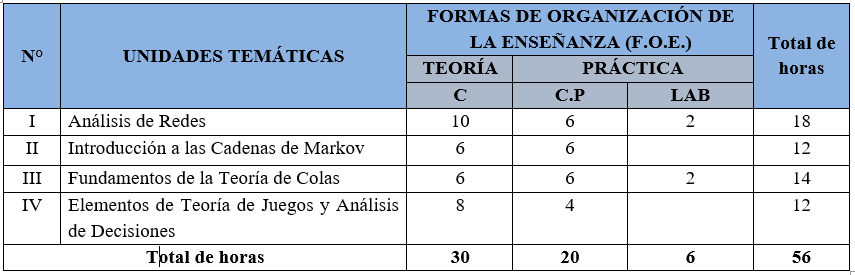
\includegraphics[scale=.5]{images/plan_tematico.png}
\end{center}
\end{frame}

\section{Unidad 1: Análisis de Redes}
\begin{frame}
\frametitle{Objetivos de la Unidad 1}
\begin{itemize}
    \item \textbf{Conceptual}:  Comparar los distintos algoritmos para la resolución de un problema de red considerando la formulación y las restricciones del problema.
    \item \textbf{Procedimental}: Utilizar la información recopilada de la red para presentar las alternativas de solución interpretando los parámetros calculados en la resolución del problema.
    \item \textbf{Actitudinal}: Valorar los resultados obtenidos de sus modelos, comparando con las aplicaciones existentes sobre redes de las empresas radicadas en el país.
\end{itemize}
\end{frame}

\section{Sesión 1}
\begin{frame}
\frametitle{Sesión 1}

\textbf{Tema}
\begin{enumerate}
\item Terminología de Redes.
\begin{enumerate}
\item Redes Dirigidas y No dirigidas
\item  Trayectoria. Trayectoria Dirigida.
\item  Red Conexa
\item Nodos Fuentes, Intermedio y de Transbordo.
\end{enumerate}
\end{enumerate}
\textbf{Objetivo}
\begin{itemize}
    \item El estudiante identificará la terminología de redes, incluyendo redes dirigidas y no dirigidas, trayectorias, redes conexas y tipos de nodos, mediante el análisis de conceptos y ejemplos aplicados, para comprender su importancia en la modelización de problemas ingenieriles.
\end{itemize}
\end{frame}

% Diapositiva
\begin{frame}
    \frametitle{Modelos de Flujo en Redes}
    
    \begin{itemize}
        \item Muchas operaciones están relacionadas con el \textbf{transporte} de elementos en una \textbf{red}.
        \begin{itemize}
            \item Movimiento de materiales desde proveedores a fábricas.
            \item Transporte de bienes desde fábricas a centros de distribución.
            \item Distribución de bienes desde centros de distribución a tiendas minoristas.
            \item Transporte de pasajeros a través de ferrocarriles o vuelos.
            \item Envío de paquetes de datos en Internet.
            \item Transporte de agua a través de tuberías.
        \end{itemize}
        \item Un modelo unificado, el \textbf{flujo de costo mínimo} (\textbf{MCNF}), cubre muchas operaciones en redes.
        \item Posee interesantes propiedades teóricas.
        \item También se puede utilizar para tomar decisiones sobre inventario, gestión de proyectos, asignación de trabajos, ubicación de instalaciones, etc.
    \end{itemize}

\end{frame}

\begin{frame}
    \frametitle{Redes}
    
    \begin{itemize}
        \item Una \textbf{red} (grafo) tiene \textbf{nodos} (vértices) y \textbf{arcos} (aristas/enlaces).
        \begin{itemize}
            \item Una interpretación típica: Los nodos representan ubicaciones y los arcos representan caminos.
        \end{itemize}
    \end{itemize}
    
    \begin{center}
        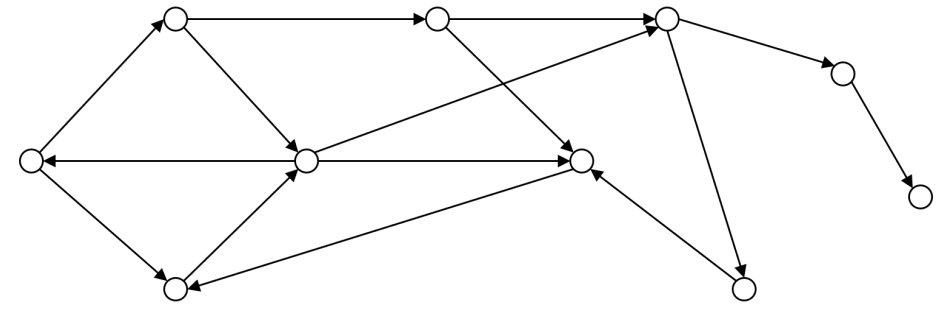
\includegraphics[width=0.8\textwidth]{images/network_graph.png} % Asegúrate de cambiar el nombre de la imagen si es necesario.
    \end{center}
    
    \begin{itemize}
        \item Los arcos pueden ser \textbf{dirigidos} o \textbf{no dirigidos}.
        \begin{itemize}
            \item Un arco de $u$ a $v$: $(u,v)$ si es dirigido y $[u,v]$ si es no dirigido.
            \item En esta presentación, todos los arcos son dirigidos.
            \item Una red es dirigida si todos sus arcos son dirigidos.
            \item Una red no dirigida también se conoce como grafo (según algunas personas).
        \end{itemize}
    \end{itemize}

\end{frame}

\begin{frame}
    \frametitle{Caminos y Ciclos}
    
    \begin{itemize}
        \item Un \textbf{camino} (ruta) desde el nodo $s$ hasta el nodo $t$ es un conjunto de arcos:
    \end{itemize}
    
    \begin{center}
        $(s,v_1), (v_1,v_2), \dots, (v_{k-1},v_k), \text{ y } (v_k,t)$
    \end{center}
    
    \begin{itemize}
        \item De manera que $s$ y $t$ están \textbf{conectados}.
    \end{itemize}
    \vspace{-.5cm}
    \begin{center}
        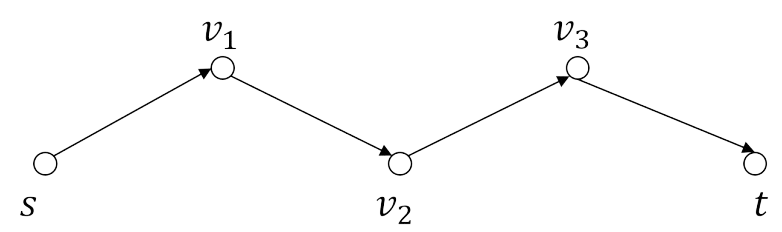
\includegraphics[width=0.8\textwidth]{images/path_cycle_graph.png} % Asegúrate de cambiar el nombre de la imagen si es necesario.
    \end{center}
    \vspace{-.5cm}
    \begin{itemize}
        \item $s$ se llama la \textbf{fuente} y $t$ se llama el \textbf{destino} del camino. ¡La dirección importa!
        \item Un \textbf{ciclo} es un camino cuyo nodo de destino es el nodo de origen.
        \item Un camino es un \textbf{camino simple} si no es un ciclo.
        \item Una red es una \textbf{red acíclica} si no contiene ciclos.
    \end{itemize}

\end{frame}


\begin{frame}
    \frametitle{Flujos, Pesos y Capacidades}
    
    \begin{itemize}
        \item Un \textbf{flujo} en un arco es la acción de enviar elementos a través del arco.
        \begin{itemize}
            \item La cantidad de unidades enviadas se llama \textbf{tamaño del flujo}.
        \end{itemize}
        \item Un \textbf{flujo en red} es la colección de todos los flujos en los arcos.
        \begin{itemize}
            \item Un flujo en red es simplemente un plan para establecer flujos en todos los arcos.
        \end{itemize}
        \item Un arco puede tener un \textbf{peso}.
        \begin{itemize}
            \item Un peso puede representar una distancia, un costo por unidad de flujo, etc.
        \end{itemize}
        \item Una \textbf{red ponderada} es una red cuyos arcos tienen pesos.
        \item Un arco puede tener una \textbf{restricción de capacidad}.
        \begin{itemize}
            \item Puede haber un límite superior y/o un límite inferior (típicamente 0) para su tamaño de flujo.
        \end{itemize}
        \item Una red es \textbf{capacitadas} si hay algún arco con límites de capacidad.
    \end{itemize}

\end{frame}

\begin{frame}
    \frametitle{Problema de Flujo en Redes de Costo Mínimo}
    
    \begin{itemize}
        \item Consideremos una red ponderada y capacitada $G = (V, E)$.
        \begin{itemize}
            \item $G$ es la red, $V$ es el conjunto de nodos y $E$ es el conjunto de arcos.
        \end{itemize}
        \item Para un nodo $i \in V$, existe una \textbf{cantidad de suministro} $b_i$.
        \begin{itemize}
            \item $b_i > 0$: $i$ es un nodo de \textbf{suministro}.
            \item $b_i < 0$: $i$ es un nodo de \textbf{demanda}.
            \item $b_i = 0$: $i$ es un nodo de \textbf{transbordo}.
            \item $\sum_{i \in V} b_i = 0$: La oferta total es igual a la demanda total.
        \end{itemize}
        \item Para un arco $(i,j) \in E$, el peso $c_{ij} \geq 0$ representa el \textbf{costo} de cada unidad de flujo.
        \item ¿Cómo \textbf{satisfacer toda la demanda} enviando un flujo de \textbf{costo mínimo} desde los nodos de suministro?
        \item Esto se conoce como el problema de \textbf{flujo en redes de costo mínimo} (MCNF).
    \end{itemize}

\end{frame}

\begin{frame}
    \frametitle{Un Ejemplo}
    
    \begin{center}
        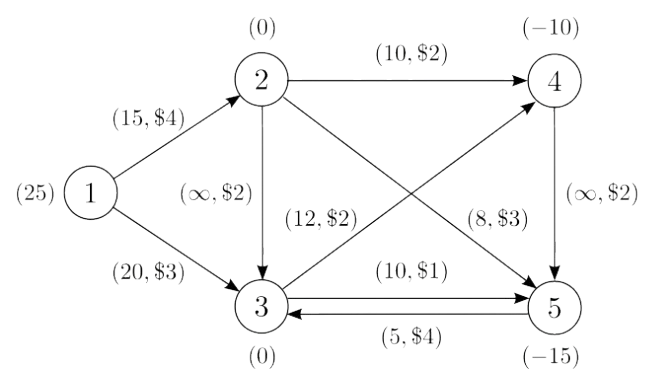
\includegraphics[width=0.6\textwidth]{images/network_example.png} % Asegúrate de cambiar el nombre de la imagen si es necesario.
    \end{center}
    
    \begin{itemize}
        \item Para cada nodo $i$, la etiqueta $(b_i)$ representa su cantidad de suministro $b_i$.
        \begin{itemize}
            \item Un nodo de suministro, dos nodos de demanda y dos nodos de transbordo.
        \end{itemize}
        \item Para cada arco $(i,j)$, la etiqueta $(u_{ij}, c_{ij})$ indica que su capacidad superior de flujo es $u_{ij}$ y su costo por unidad de flujo es $c_{ij}$.
        \begin{itemize}
            \item Algunos arcos pueden tener capacidad ilimitada.
            \item Entre dos nodos pueden existir dos arcos en direcciones opuestas.
        \end{itemize}
        \item ¿Existe algún \textbf{flujo factible}?
    \end{itemize}

\end{frame}

\begin{frame}
\frametitle{Preguntas}
\centering
\Huge{¿Preguntas?}
\end{frame}

\end{document}
